%!TeX root=../main.tex
\فصل{سنسورها}


\قسمت{مقدمه} 

به‌منظور استخراج داده‌های جوی نظیر دمای هوا، رطوبت، فشار، شدت نور و... از سنسورهای دیجیتال استفاده می‌شود. این سنسورها علاوه بر کم‌مصرف بودن دارای دقت بالا و تأخیر پایینی در اندازه‌گیری پارامترهای موردنظر هستند. با دارا بودن این ویژگی‌ها این سنسورها کاملاً با سیستم تغذیه باتری و سلول خورشیدی سازگار هستند.

‌\قسمت{فشارسنج}

تغییرات فشار جوی یکی از عناصر مهم در پیش‌بینی وضعیت آب‌وهوا است. فشارسنج‌های جیوه‌ای از اواخر قرن 16 جهت پیش‌بینی وضعیت آب‌وهوا مورداستفاده قرار می‌گرفت. به‌طورکلی تغییر فشار هوا رو به بالا نشان‌دهنده آسمان آفتابی، گرم و صاف و تغییر فشار هوا رو به پایین نشان‌دهنده بارش باران، طوفان و آسمانی مملو از ابرهای باران‌زا است. علاوه بر این فشار هوا یکی از عوامل مؤثر در سنجش سرعت باد نیز به شمار می‌آید. 

سنسور استفاده‌شده برای این منظور ماژول سنسور \متن‌لاتین{BMP180} است که با مصرف جریان تنها در حد چند میکرو آمپر دقتی معادل با 0٫3 هکتوپاسکال\پانویس{Hectopascal (hPa)} دارد و توانایی اندازه‌گیری فشار هوا در بازه 300 تا 1100 هکتوپاسکال را دارا است. نحوه ارتباط با این ماژول از طریق رابط \متن‌لاتین{I\بالانویس‌متنی{2}C} است. تصویر رو و پشت این ماژول در شکل \رجوع{fig:BMP180} آمده است.

\begin{figure}[!h]
	\begin{subfigure}{0.5\linewidth}
		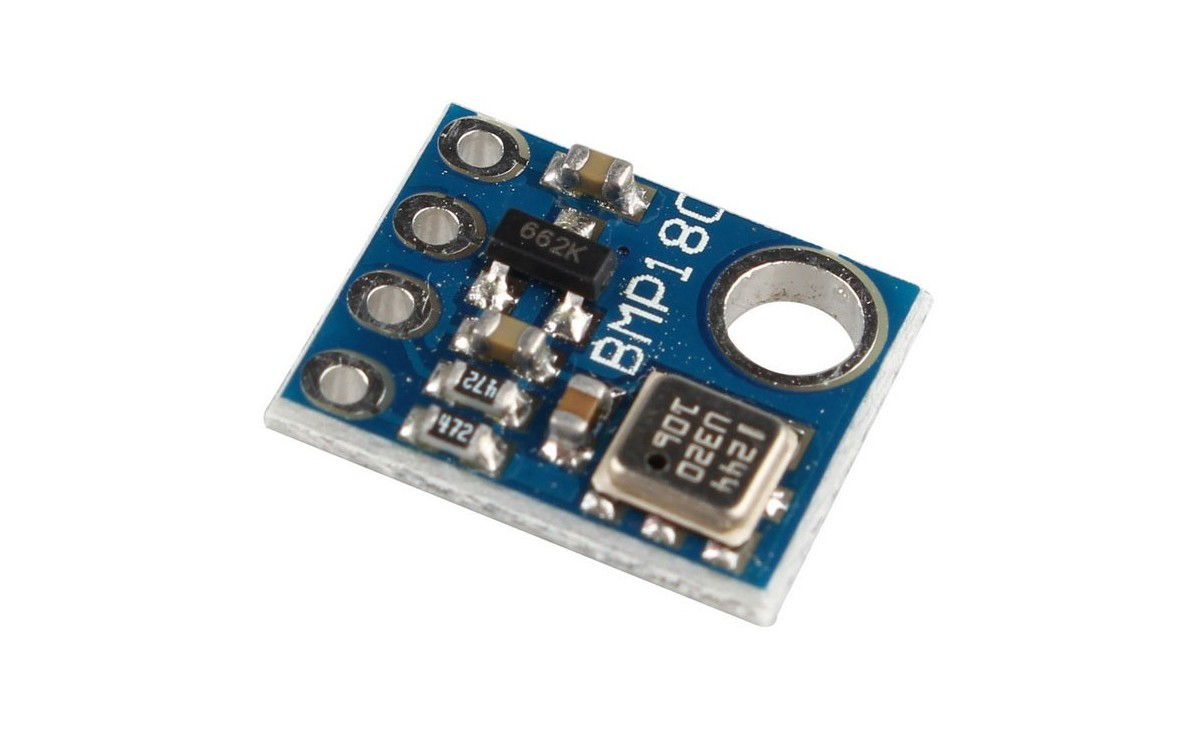
\includegraphics[width=\linewidth]{Assets/BMP180front.jpg}
		\caption{تصویر روی ماژول \متن‌لاتین{BMP180}.}
		\label{fig:BMP180front}
	\end{subfigure}
	\begin{subfigure}{0.5\linewidth}
		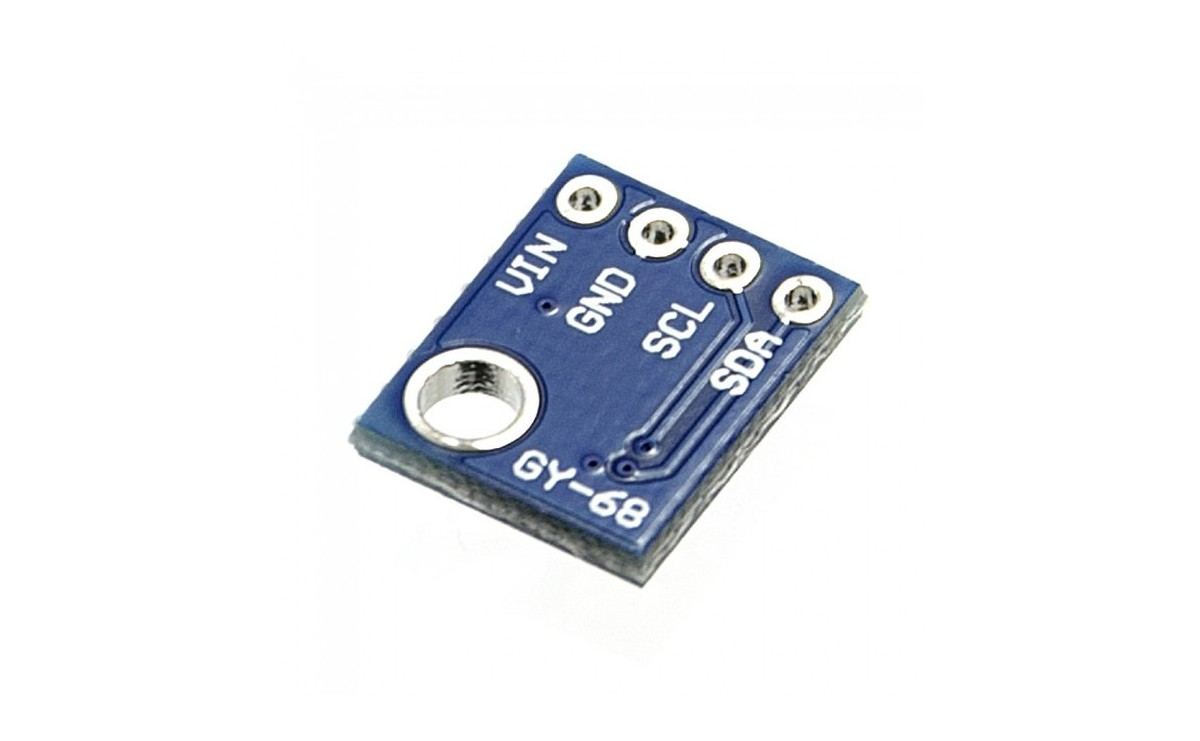
\includegraphics[width=\linewidth]{Assets/BMP180back.png}
		\caption{تصویر پشت ماژول \متن‌لاتین{BMP180}.}
		\label{fig:BMP180back}
	\end{subfigure}
	\caption{تصویر پشت و روی ماژول \متن‌لاتین{BMP180}.}
	\label{fig:BMP180}
\end{figure}

‌\قسمت{شدت نور}

شدت نور خورشید یکی از پارامترهای اصلی سنجش وضعیت آب‌وهوا است. از این سنسور جهت نشخیص ابری یا آفتابی بودن هوا می‌توان استفاده کرد. همچنین به دلیل اهمیت موضوع سلامت پوست، معمولاً در کنار این سنسور از سنسور سنجش شدت \متن‌لاتین{UV} به‌منظور اطلاع‌رسانی شدت \متن‌لاتین{UV} نیز استفاده می‌شود. 

جهت سنجش شدت نور از ماژول سنسور \متن‌لاتین{MAX44009} استفاده‌شده است که با 0٫65 میکرو آمپر مصرف جریان در هنگام کارکرد شدت نور در بازه‌ی 0٫045 لوکس تا 188 هزار لوکس را اندازه‌گیری می‌کند. همچنین اینترفیس ارتباطی این ماژول رابط سریالی \متن‌لاتین{I\بالانویس‌متنی{2}C} می‌باشد. تصویر رو و پشت این ماژول در شکل \رجوع{fig:MAX44009} آمده است.

\begin{figure}[H]
	\centering
	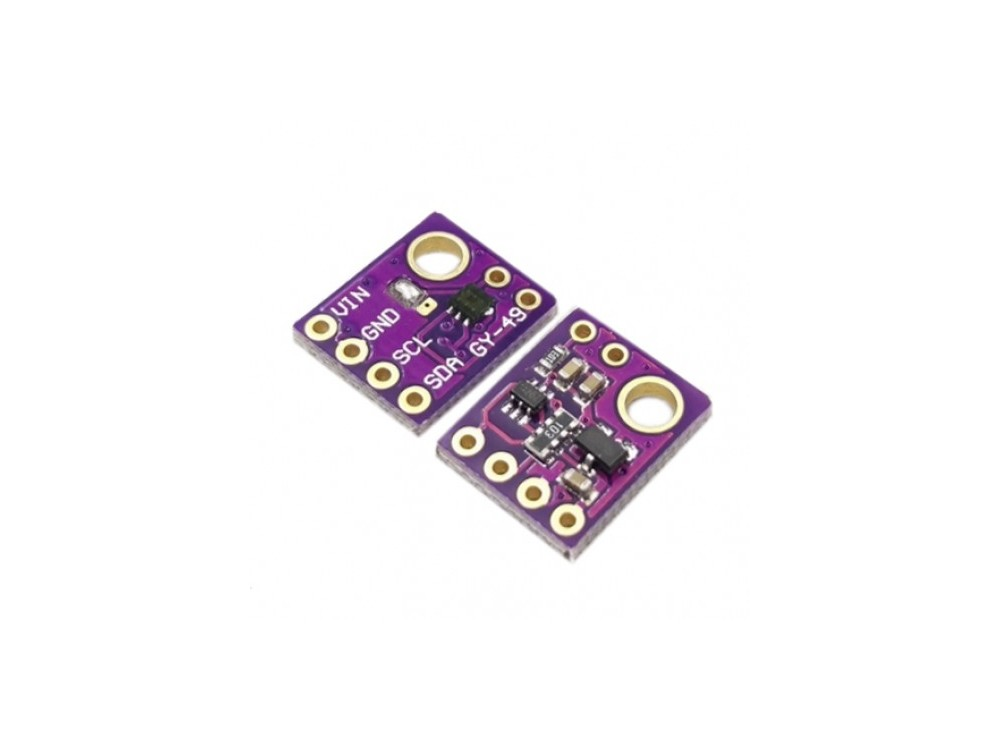
\includegraphics[width=0.8\linewidth]{Assets/MAX44009.jpg}
	\caption{تصویر پشت و روی ماژول \متن‌لاتین{MAX44009}.}
	\label{fig:MAX44009}
\end{figure}

‌\قسمت{قطب‌نما}

ازآنجایی‌که این دستگاه در سمت سنسور معمولاً در ارتفاع 10 متری زمین روی یک میله نصب می‌شود، قرار دادن دستگاه در جهت جغرافیایی خاص، به جهت سنجش جهت باد، ممکن است دشوار باشد (یا حتی خیلی دقیق نباشد). باوجود سنسور قطب‌نما در این دستگاه (برخلاف برخی دستگاه‌های مشابه) دیگر نیازی به نصب دستگاه در جهت جغرافیایی خاص نخواهد بود.

سنسور استفاده‌شده برای این منظور سنسور \متن‌لاتین{QMC5883L} است. که با ماکسیموم 100 میکرو آمپر جریان مصرفی می‌توان به‌دقت یک تا دو درجه در جهت‌یابی رسید. همچنین طریقه ارتباط این سنسور با میکروکنترلر از طریق رابط \متن‌لاتین{I\بالانویس‌متنی{2}C} است. تصویر رو و پشت این ماژول در شکل \رجوع{fig:QMC5883L} آمده است.

\begin{figure}[!h]
	\begin{subfigure}{0.5\linewidth}
		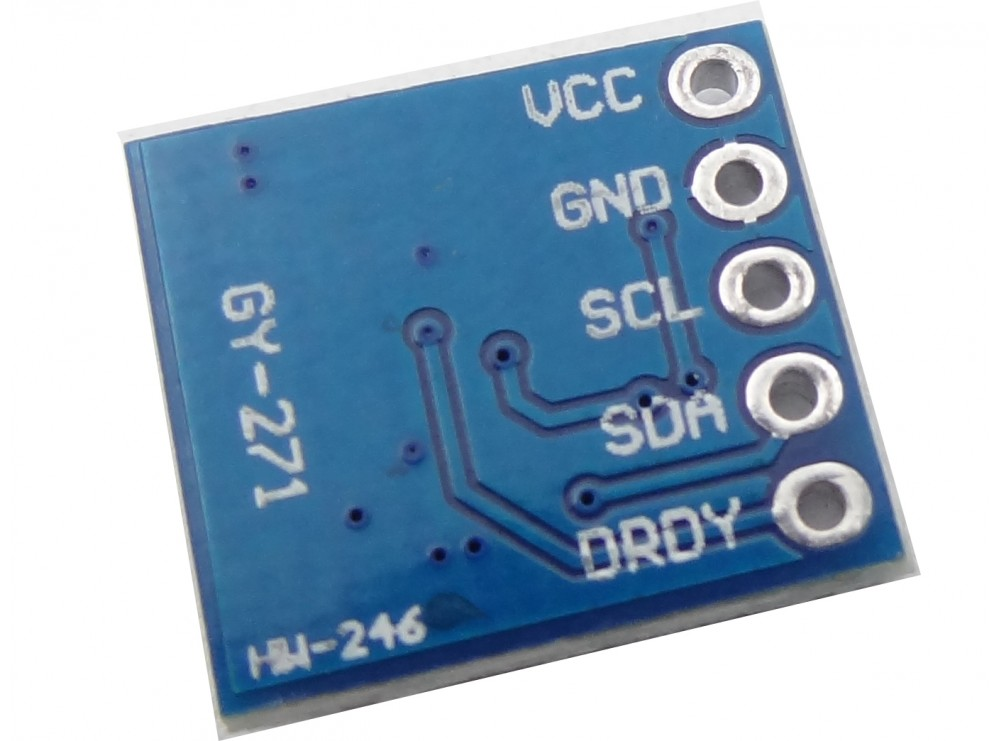
\includegraphics[width=\linewidth]{Assets/QMC5883Lback.jpg}
		\caption{تصویر پشت ماژول \متن‌لاتین{QMC5883L}.}
		\label{fig:BMP180back}
	\end{subfigure}
	\begin{subfigure}{0.5\linewidth}
		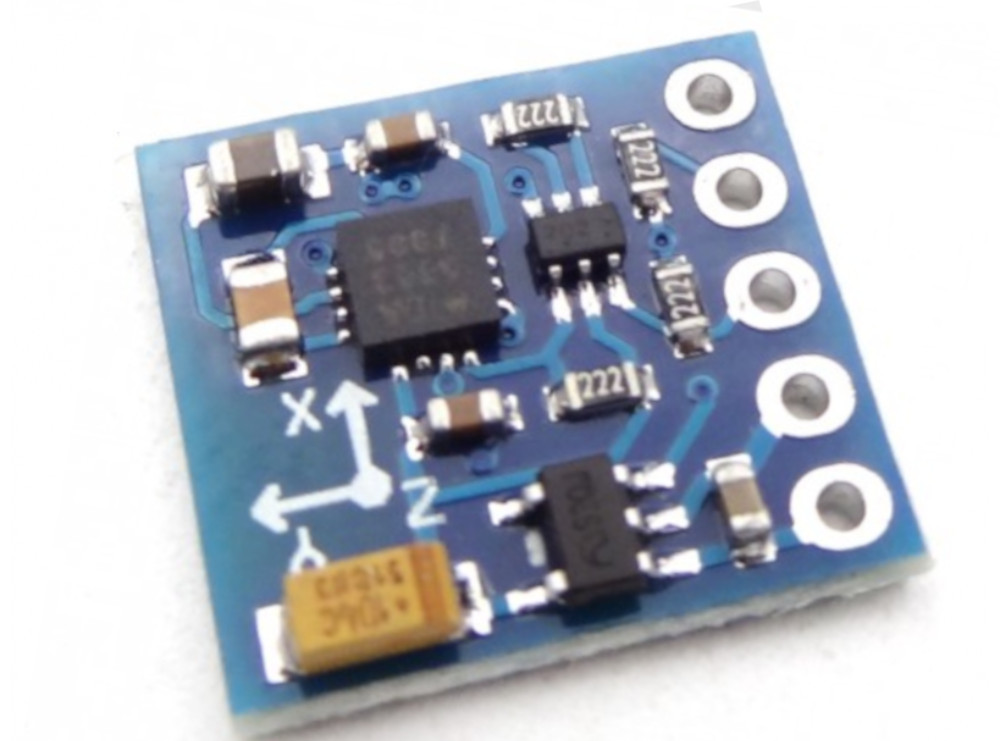
\includegraphics[width=\linewidth]{Assets/QMC5883Lfront.jpg}
		\caption{تصویر روی ماژول \متن‌لاتین{QMC5883L}.}
		\label{fig:QMC5883Lfront}
	\end{subfigure}
	\caption{تصویر پشت و روی ماژول \متن‌لاتین{QMC5883L}.}
	\label{fig:QMC5883L}
\end{figure}

‌\قسمت{دما و رطوبت هوا}

درکتار وضعیت آسمان (ابری، آفتابی، بارانی و... بودن) معمولاً به‌طور مستقیم پارامتر دمای هوا نیز در اطلاع‌رسانی وضعیت و پیش‌بینی آب‌وهوا نقش ایفا می‌کند. در کنار این موارد رطوبت هوا نیز، علاوه بر نقشی که در پیش‌بینی دارد، معمولاً به‌طور مستقیم به سمع و نظر مخاطبین می‌رسد. علاوه این رطوبت نسبی هوا در کنار دمای هوا نقش مهمی در رسیدن به آسایش حرارتی در بدن انسان (و موجودات) دارد. به‌طوری کلی در دمای هوای بالاتر به رطوبت نسبی کمتری نسبت به دمای هوای پایین‌تر برای رسیدن به سطح آسایش  حرارتی نیاز است \مرجع{Schiavon2013}. 

ماژول سنسور \متن‌لاتین{AHT10} دما و رطوبت نسبی هوا را با دقت 0٫01 درجه سلسیوس\پانویس{Celsius} و 0٫024 درصد با تنها 3٫3 میکرو وات مصرف توان اندازه‌گیری می‌کند. همچنین این ماژول در رطوبت 0 تا 100 درصد و دمای  40- تا 100 درجه‌ی سلسیوس قابل‌استفاده است. خروجی این ماژول نیز سیگنال دیجیتال ارتباطی \متن‌لاتین{I\بالانویس‌متنی{2}C} است. تصویر رو و پشت این ماژول در شکل \رجوع{fig:AHT10} آمده است.

\begin{figure}[H]
	\begin{subfigure}{0.5\linewidth}
		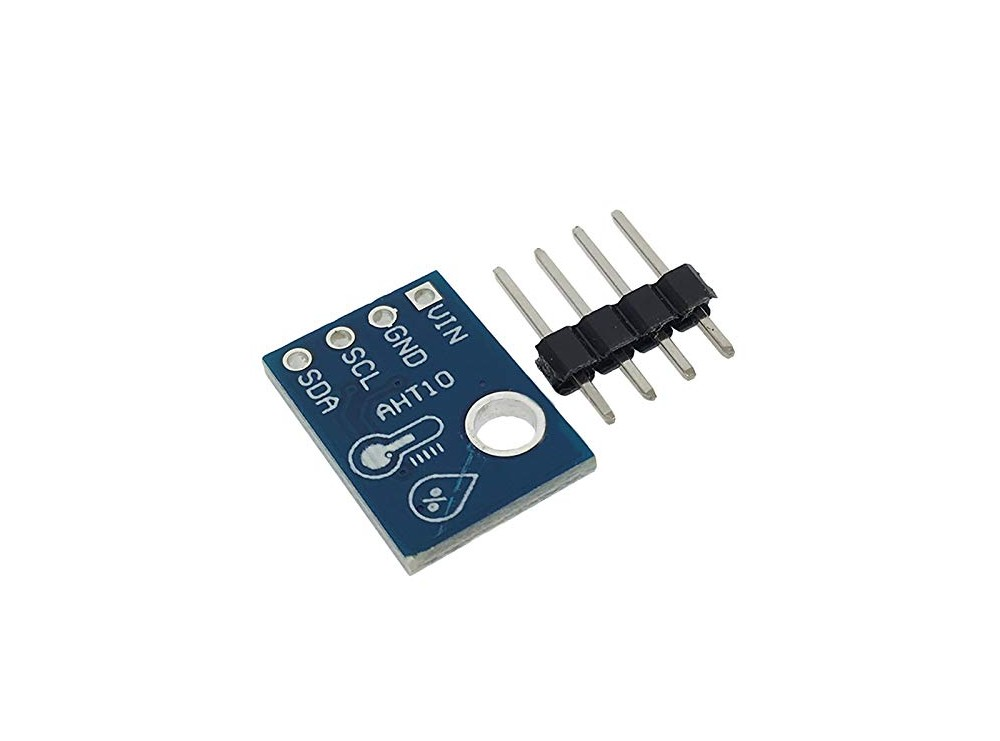
\includegraphics[width=\linewidth]{Assets/AHT10back.jpg}
		\caption{تصویر پشت ماژول \متن‌لاتین{AHT10}.}
		\label{fig:AHT10}
	\end{subfigure}
	\begin{subfigure}{0.5\linewidth}
		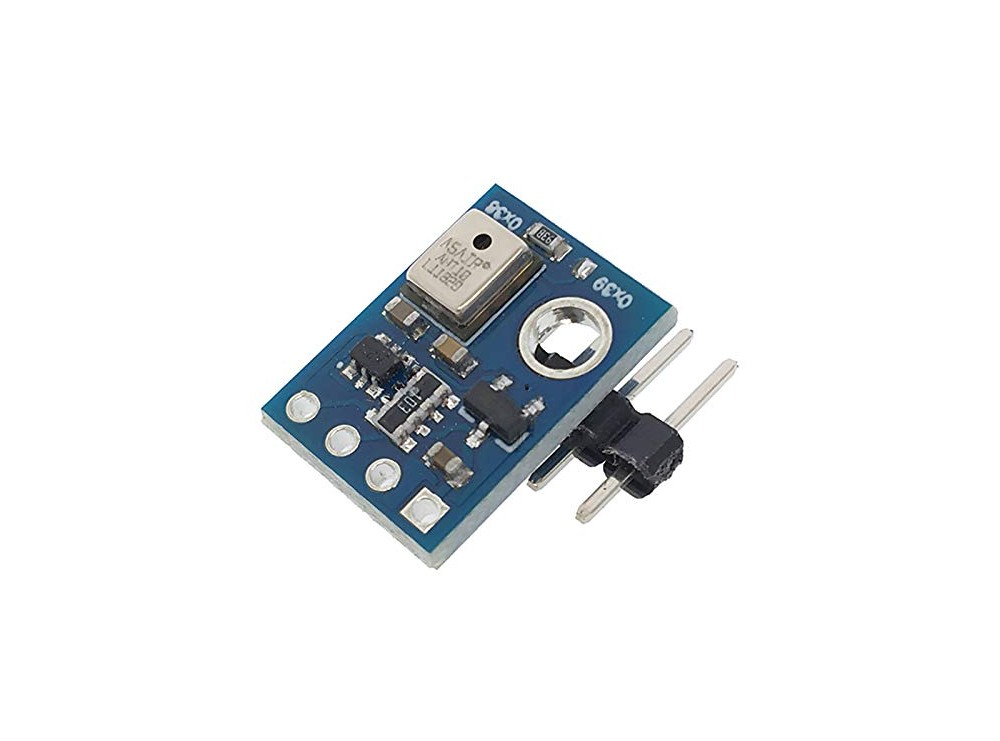
\includegraphics[width=\linewidth]{Assets/AHT10front.jpg}
		\caption{تصویر روی ماژول \متن‌لاتین{AHT10}.}
		\label{fig:AHT10}
	\end{subfigure}
	\caption{تصویر پشت و روی ماژول \متن‌لاتین{AHT10}.}
	\label{fig:AHT10}
\end{figure}

‌\قسمت{شدت و جهت باد}\label{sec:windSpeedANDAngle}

روش‌های مختلفی برای سنجش شدت باد وجود دارد، عمدتاً در این کاربرد دو روش سنجش مکانیکی و آلتراسونیک \پانویس{Ultrasonic} مورداستفاده قرار می‌گیرد. در سنجش شدت و جهت باد در روش مکانیکی از دو ابزار که به‌صورت مستقل کار می‌کنند (در برخی موارد این دو ابزار در قالب یک دستگاه در کنار هم قرار می‌گیرند) استفاده می‌شود، به طوری که یک ابزار برای سنجش شدت و ابزاری دیگر برای تعیین جهت، مورداستفاده قرار می‌گیرد. هر دو دستگاه دارای قطعات متحرک‌اند و یکی با داشتن پره‌هایی شبیه به دم هلی‌کوپتر با وزرش باد در جهت وزش قرار می‌گیرد و دیگری دارای پره‌هایی است که با وزش باد پره‌ها همانند پره‌های توربین به حرکت درمی‌آید که با توجه به‌سرعت چرخش پره‌ها سرعت باد قابل‌اندازه‌گیری است. در اندازه‌گیری‌های این دستگاه‌ها محدودیت‌هایی وجود دارد و اغلب این نوع ابزارها در وزش باد ملایم عملکرد صحیحی از خود نشان نمی‌دهند. همچنین در اندازه‌گیری زاویه وزش ممکن‌ است محدود به اندازه گیری زوایای خاصی باشند. 

در روش اندازه‌گیری شدت و جهت باد با آلتراسونیک اندازه‌گیری‌ها می‌تواند در قالب تنها یک دستگاه، بدون قطعات متحرک و با دقتی بالاتر انجام پذیرد. در این روش 2 فرستنده و گیرنده آلتراسونیک همان‌طور که در شکل \رجوع{fig:oneAxisUltrasonic} نشان داده‌شده است روبروی یکدیگر در فاصله مشخص $d$ قرار داده می‌شوند.

\begin{figure}[!h]
	\centering
	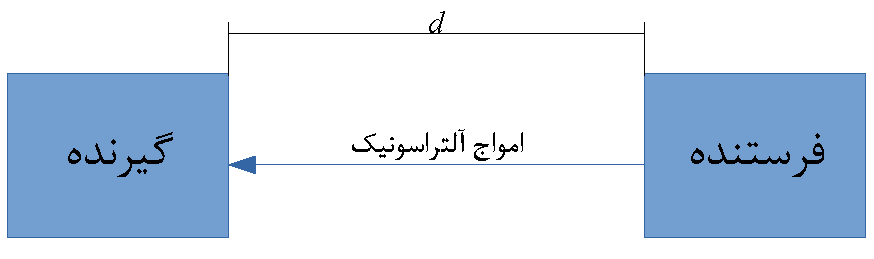
\includegraphics[width=0.6\linewidth]{Assets/ultrasonic one axis.pdf}
	\caption{نحوه قرارگیری فرستنده و گیرنده آلتراسونیک.}
	\label{fig:oneAxisUltrasonic}
\end{figure}

فرستنده امواج صوتی با فرکانس 40 کیلوهرتز (که برای گوش انسان قابل شنیدن نیست) تولید می‌کند. فاصله زمانی بین ارسال امواج صوتی از فرستنده و دریافت این امواج در گیرنده اندازه‌گیری می‌شود. با توجه به رابطه \رجوع{eq:speed}، سرعت $v$ با داشتن فاصله $d$ و زمان تأخیر بین ارسال موج صوتی در فرستنده و دریافت آن در گیرنده  $t$، قابل‌اندازه‌گیری است.

\begin{equation}\label{eq:speed}
v = \frac{d}{t}
\end{equation}

سرعت $v$ به‌دست آمده از این رابطه مطابق رابطه \رجوع{eq:expandSpeed} متشکل از سرعت صوت $v_s$ و سرعت باد $v_{wx}$  است \مرجع{7988049}.

\begin{equation}\label{eq:expandSpeed}
v = v_s + v_{wx}
\end{equation}

درصورتی‌که وزش باد در جهت موافق حرکت امواج صوتی باشد زمان تأخیر در دریافت امواج نسبت به حالی که باد نوزد کمتر شده و درنتیجه سرعت $v$ نسبت به حالتی که باد نوزد افزایش می‌یابد (یعنی علامت $v_{wx}$ مثبت بوده و $v = v_s+v_{wx}$). درصورتی‌که وزش باد در خلاف جهت حرکت امواج صوتی باشد زمان تأخیر در دریافت امواج نسبت به حالتی که باد نوزد بیشتر شده و درنتیجه سرعت $v$ کاهش می‌یابد (یعنی علامت $v_{wx}$ منفی بوده و $v = v_s-v_{wx}$). با داشتن سرعت صوت $v_s$، فاصله $d$ و محاسبه زمان $t$ می‌توان با توجه به معادلات \رجوع{eq:speed} و \رجوع{eq:expandSpeed} سرعت باد $v_{wx}$ و جهت باد (علامت سرعت $v_{wx}$) روی یک محور مطابق رابطه \رجوع{eq:speedWindX} به‌دست آورد. 

\begin{equation}\label{eq:speedWindX}
v_{wx} = \frac{d}{t} - v_s
\end{equation}

به‌منظور سنجش شدت و جهت باد در دو بعد می‌توان دو فرستنده و گیرنده دیگر بر روی محوری عمود بر محور متصل‌کننده فرستنده و گیرنده فعلی قرارداد و با محاسبه دو بردار سرعت، بردار سرعت برآیند را به‌دست آورد.
\begin{figure}[!h]
	\centering
	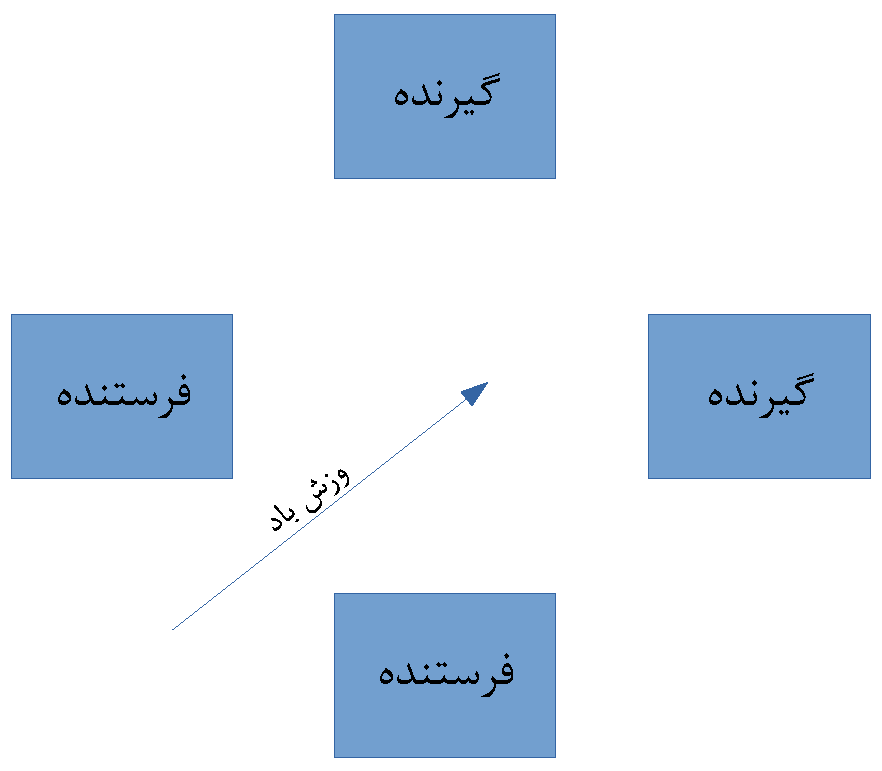
\includegraphics[width=0.7\linewidth]{Assets/ultrasonic 2d.pdf}
	\caption{نحوه قرارگیری فرستنده و گیرنده آلتراسونیک دو محوره.}
	\label{fig:2dUltrasonic}
\end{figure}

\begin{figure}[!h]
	\centering
	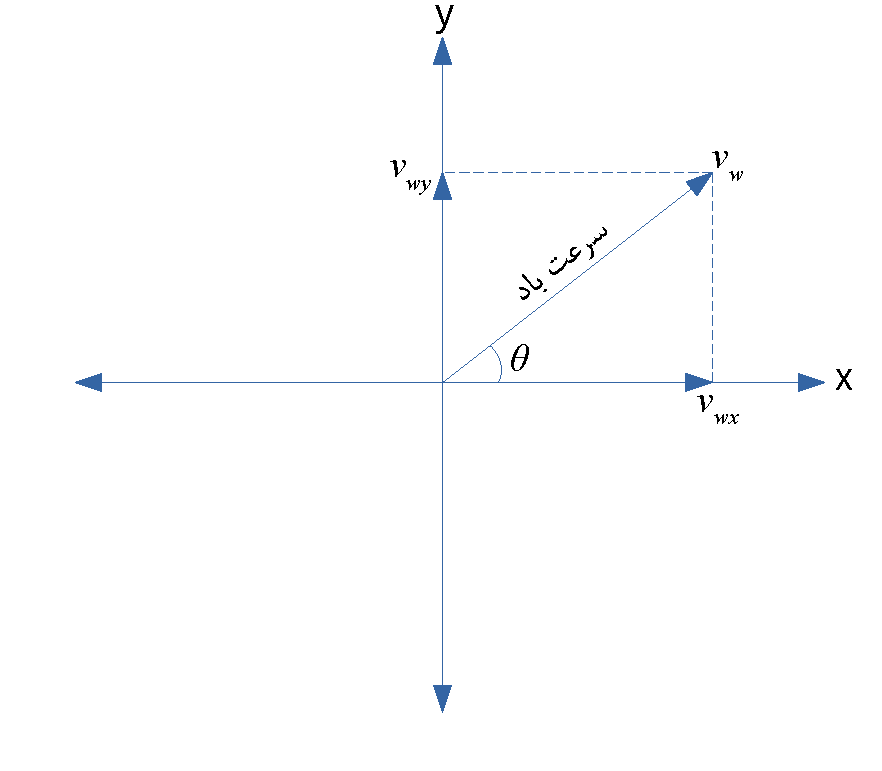
\includegraphics[width=0.7\linewidth]{Assets/ultrasonic 2d axis.pdf}
	\caption{ بردار‌های متناظر با نحوه قرارگیری فرستنده و گیرنده آلتراسونیک دو محوره.}
	\label{fig:2dUltrasonicAxis}
\end{figure}

اگر نحوه قرارگیری فرستنده و گیرنده‌ها مطابق شکل \رجوع{fig:2dUltrasonic} باشد در این صورت صفحه مختصات متناظر با آن مطابق شکل \رجوع{fig:2dUltrasonicAxis} خواهد بود. اندازه $v_w$ و زاویه $\theta$ بردار سرعت باد از طریق روابط \رجوع{eq:windSpeed} به‌دست می‌آیند.

\begin{equation}\label{eq:windSpeed}
\begin{split}
v_w = \sqrt{v_{wx}^2 + v_{wy}^2}\\
\theta = \tan^{-1}{\left( \frac{v_{wy}}{v_{wx}}\right)}
\end{split}	
\end{equation}

\begin{table}[!t]
	\centering
	\caption{ضرایب  محاسبه سرعت صوت (فرمول \رجوع{eq:soundSpeed}) \مرجع{cramer1993variation}.}
	\label{tb:speedOfSoundcoefficients}
	\begin{tabular}{cc}
		\hline \hline
		ضرایب & \\
		\hline
		$a_{0}$ & $331.5024$ \\
		$a_{1}$ & $0.603055$ \\
		$a_{2}$ & $-0.000528$ \\
		$a_{3}$ & $51.471935$ \\
		$a_{4}$ & $0.1495874$ \\
		$a_{5}$ & $-0.000782$ \\
		$a_{6}$ & $-1.82 \times 10^{-7}$ \\
		$a_{7}$ & $3.73 \times 10^{-8}$ \\
		$a_{8}$ & $-2.93 \times 10^{-10}$ \\
		$a_{9}$ & $-85.20931$ \\
		$a_{10}$ & $-0.228525$ \\
		$a_{11}$ & $5.91 \times 10^{-5}$ \\
		$a_{12}$ & $-2.835149$ \\
		$a_{13}$ & $-2.15 \times 10^{-13}$ \\
		$a_{14}$ & $29.179762$ \\
		$a_{15}$ & $0.000486$ \\
		\hline
	\end{tabular}
\end{table}

سرعت صوت $v_s$ به‌عنوان تابعی از دما، فشار و کسر مولی رطوبت و کربن دی‌اکسید، با استفاده از رابطه \رجوع{eq:soundSpeed} قابل‌محاسبه است \مرجع{cramer1993variation}. ثوابت$a_1$ تا $a_{15}$ در جدول \رجوع{tb:speedOfSoundcoefficients} آمده‌اند.

\begin{equation}\label{eq:soundSpeed}
\begin{aligned}
v_s\left(\tau, p, x_w, x_{c}\right)=& a_{0}+a_{1} \tau+a_{2} \tau^{2}+\left(a_{3}+a_{4} \tau+a_{5} \tau^{2}\right) x_{w} \\
&+\left(a_{6}+a_{7} \tau+a_{8} \tau^{2}\right) p+\left(a_{9}+a_{10} \tau+a_{11} \tau^{2}\right) x_{c} \\
&+a_{12} x_{w}^{2}+a_{13} p^{2}+a_{14} x_{c}^{2}+a_{15} x_w p x_c
\end{aligned}
\end{equation}

که $\tau$ دمای هوا (برحسب درجه سلسیوس)، $p$ فشار هوا (برحسب پاسکال)، $x_w$ کسر مولی بخارآب در هوا و $x_c$ کسر مولی کربن دی‌اکسید در هوا است. $x_c$ را ثابت و برابر $400 \times 10^{-6}$ در نظر می‌گیریم. کسر مولی بخارآب در هوا $x_w$ از رابطه \رجوع{eq:x_w} به‌دست می‌آید \مرجع{rasmussen1997calculation}. 

\begin{equation}\label{eq:x_w}
x_w=\frac{h f p_{sv}}{100 p}
\end{equation}

که $h$ درصد رطوبت هوا، $p_{sv}$ فشار اشباع بخارآب در هوا و $f$ ضریب تقویت است و از طریق روابط \رجوع{eq:f} و \رجوع{eq:p_sv} محاسبه می‌شوند \مرجع{davis1992equation}.

\begin{equation}\label{eq:f}
f=1.00062+3.14 \times 10^{-8} p+5.6 \times 10^{-7} \tau^{2}
\end{equation}
\begin{equation}\label{eq:p_sv}
\begin{aligned}
p_{s v}=& \exp \left(1.2811805 \times 10^{-5} T^{2}-1.9509874 \times 10^{-2} T\right.\\
&\left.+34.04926034-6.3536311 \times 10^{3} / T\right)
\end{aligned}
\end{equation}

که در این روابط $T$ دمای محیط برحسب کلوین\پانویس{Kelvin} است، یعنی:
\begin{equation}
T = \tau + 273.15
\end{equation}
